
\chapter{Bibliothèque Scheme}
%% Bonne place???

Le langage Scheme\cite{Scheme} à été conçu en 1975 par Guy L. Steele et Gerald
Jay Sussman.  Ces un langage de programmation avec un système de type
dynamique, cela signifie que les variables peuvent contenir n'importe quels
types. Il supporte plusieurs paradigme de programmation comme fonctionnel,
impérative et méta.

Le paradigme impératif se retrouve dans des langage comme C, dans lequel chacune
des instructions est un ordre donnée à la machine. C'est langage supporte
l'assignation de variable dans l'initialisation et dans la modification.

Dans la programmation fonctionnelle, il y a une distinction entre les opérations
pures et les opérations qui ont des effets de bord. Les opérations dite pure ont
la caractéristique que leurs résultats ne varient pas pour des mêmes entrées.
Des exemples d'opérations pures sont les opérations mathématiques. Les effets
de bord sont souvent lié aux assignation et au opération d'entrée/sortie. La programmation
méta est un paradigme relatif à l'utilisation de macro.

Une expression en syntaxe infixe place l'opérateur entre les opérande. Cette
forme est souvent utilisé  dans les langages impératif. La syntaxe préfixé
commence par l'opérateur suivie des opérandes. Cette forme est plus utilisé dans les
langages de la famille LISP.

Un programme Scheme est une séquence de liste parenthésé en forme préfixé, ce sont des \textit{s-expresssions}.
Chaque \textit{s-expression} correspond soit à une constante, une application de procédure ou une
application de macro.

\begin{verbatim}
- Scheme
  - Langage dynamique
  - Supporte plusieurs paradigmes:
    - fonctionnel
    - impérative
    - méta (programmation de macro)
  - Préfixé / ~Infixe
  - S-expression
\end{verbatim}


\begin{table}[htbp]
\begin{center}
\begin{tabular}{|l|l|}
  \hline
  \textbf{Préfixe}& \textbf{Infixe}\\\hline
  \begin{mplisting}{0.1}
(+ 1 2)
\end{mplisting}&
  \begin{mplisting}{0.1}
1 + 2;
\end{mplisting}\\
\hline
  \begin{mplisting}{0.25}
(proc a1 a2 a3)
\end{mplisting}&
  \begin{mplisting}{0.25}
proc(a1, a2, a3);
\end{mplisting}\\
\hline
%    \begin{mplisting}{0.25}
%(if e1
%    e2
%    e3)
%\end{mplisting}&
%    \begin{mplisting}{0.25}
%if(e1)
%  e2;
%else
%  e3;
%\end{mplisting}\\
%\hline
\end{tabular}
\end{center}
  \caption{Voici des example qui montre une comparaison entre une syntaxe infixe et préfixe.}
\end{table}

La définition des associations globales est effectuée avec \lstcode{define}.  Cette
forme spécial associe un nom avec une valeur qui a un type quelconque.  Les types de
donnée disponible en Scheme sont \lstcode{boolean}, \lstcode{pair},
\lstcode{symbol}, \lstcode{number}, \lstcode{char}, \lstcode{string},
\lstcode{vector}, \lstcode{port} et \lstcode{procedure}.

Les procédures sont des objets de premier classe, cela signifie qu'ils peuvent
être manipulé comme les autres types de donnée. Ils peuvent
être passés en paramètre d'un procédure et retournés comme résultat.
Certaines fonctions -- tel que \lstcode{map}, \lstcode{fold}, etc. -- bénéficie
que les procédures sont des objets de premier classe.

\section{Procédure et Macro}

Les procédures et les fonctions sont définis par le constructeur
\lstcode{lambda} qui prend une liste d'arguments et une séquence d'au moins une
\textit{s-expression} comme corps. Lors de l'application d'une procédure chacun
des arguments est évalué puis les résultats des évaluations sont passés à la
procédure. C'est un mode de passage de paramètre par valeur.

Le langage n'offre pas de syntaxe spéciale pour les boucles, il offre une forme
de récursion sans coût mémoire, c'est la récursion en position terminale. La récursion
est utilisé pour effectué des boucles.


% \begin{figure}[ht]
%   \begin{center}
%     \begin{tabular}{|l|}
%       \hline
%     \begin{mplisting}{0.55}
% (define fact
%   (lambda (n) (if (= n 0) 1
%                   (* n (fact (- n 1))))))
% \end{mplisting}\\\hline
%     \end{tabular}
%   \end{center}
%   \label{fig:fact1}
%   \caption{Voici une implémentation de la fonction factoriel en Scheme.
%   Cela montre un exemple de récursion.}
% \end{figure}

% READ Distinguer macro procedure.
\begin{figure}[ht]
  \begin{center}
    \begin{tabular}{|l|}
      \hline
    \begin{mplisting}{0.65}
(define map
  (lambda (f lst)
    (if (pair? lst)
        (cons (f (car lst)) (map f (cdr lst)))
        lst)))
\end{mplisting}\\\hline
    \end{tabular}
  \end{center}
  \label{fig:fact1}
  \caption{Voici une implémentation de la fonction d'ordre supérieur \lstcode{map} en Scheme.
  Cela montre un exemple utilise les procédure en objets de première classe et
  aussi un exemple d'application récursive.}
\end{figure}



% La récursion est la façon dont les boucle sont faites.
La programmation méta est présente dans plusieurs langage comme C, C++, LISP,
Scheme, etc. Elle est basé sur des constructions qui transforment le code
appelé macro.  Ils sont utilisés pour ajouter des raccourcis au langage.  En C
et C++, les macros ne permettent pas de récursion se référant à elle-même.  Ils
sont limités au remplacement textuel simple. Un appel à la macro est remplacer
par le corps de celle-ci. Les macros de style LISP ont l'avantage d'avoir accès
à l'ensemble des procédure. La différence est le mode de passage de paramètre
durant l'application de la macro. Les paramètres sont passés à la macro sans
être évalués, c'est ce qu'on appelle le passage par nom.

Le résultat d'une macro est le code qui est exécuté. Le code est une
\textit{s-expression} donc une simple liste. La plupart des implémentation
de Scheme offre la forme \lstcode{define-macro} qui est l'équivalent du
\lstcode{defmacro} de LISP.

% Cette forme souffre d'un problème d'hygiène.

\begin{figure}[ht]
  \begin{tabular}{|l|}\hline
\begin{mplisting}{0.7}
(define-macro (include filename)
  (with-input-from-file
    filename
    (lambda ()
      `(begin
        ,@(read-all (current-input-port))))))
\end{mplisting}\\\hline
\end{tabular}

  \caption{Implémentation de la macro \texttt{include} qui permet l'inclusion
  d'un fichier dans un autre fichier avec la syntax \texttt{define-macro}.  La
  macro lit le contenu de fichier \textit{filename} et retourne le contenu de
  se fichier.}

  \label{fig:macro_include}
\end{figure}

Certaines implémentations de Scheme n'ont pas la forme
\lstcode{define-macro}. Il est possible d'écrire la macro
\lstcode{include} en utilisant la \lstcode{define-syntax}
et \lstcode{syntax-case} qui est standard au R5RS
\cite{Scheme:R5RS}.

\begin{figure}[ht]
  \begin{tabular}{|l|}\hline
\begin{mplisting}{0.8}
(define-syntax include
  (lambda (stx)
    (define (read-all port)
      (let loop ((rev-lst '()))
        (let ((expr (read port)))
          (if (eof-object? expr)
            (reverse rev-lst)
            (loop (cons expr rev-lst))))))
    (syntax-case stx ()
      ((_ fn)
       (let ((filename (syntax->datum #'fn)))
         (let ((content
                 (with-input-from-file
                    filename
                    (lambda ()
                      (cons
                        'begin
                        (read-all (current-input-port)))))))
           (datum->syntax stx content)))))))

\end{mplisting}\\\hline
\end{tabular}

  \caption{Implémentation de la macro \texttt{include} qui permet l'inclusion
  d'un fichier dans un autre fichier avec la syntax \texttt{define-syntax}.
  Cette macro effectue la même action que celle définit dans la figure
  \ref{fig:macro_include}.}

\end{figure}



%% XXX: suite 2.
La structure des bibliothèque définit dans le depuis le standard
R4RS\cite{Scheme:R4RS} et R5RS\cite{Scheme:R5RS} consistait simplement de
fichiers Scheme qui sont importés dans le module courant. Cette importation est
effectué soit par la procédure \texttt{load}. La plupart des implémentation de
Scheme on la forme spéciale \texttt{include} qui peut
Ce modèle de bibliothèque possède plusieurs lacunes.

%% Gambit doc
\begin{itemize}
  \item Ce modèle de chargement n'est pas à l'abri des chargements multiples
    d'un module qui amène soit la duplication de code ou la réévaluation
    non désiré d'un code.

  \item Toutes les déclarations dans un module sont ajoutés à l'environnement
    global lors de l'importation. Cela amène des conflits de nom entre les
    symboles du module principale et les modules importés.

  \item L'importation d'un module par \texttt{load} nécessite le chemin exacte
    du module à importer qui peut être soit relatif ou absolu.  Un chemin
    relatif prend comme origine le répertoire présent.  L'importation d'un
    module par \texttt{include}, contrairement au \texttt{load}, le chemin
    relatif prend comme origine l'emplacement du fichier dans lequel la forme
    spécial \texttt{include} ce situe.

\end{itemize}


Lors d'un chargement de bibliothèque par \texttt{load} les macros sont expansé
et le code résultant est exécuté. Pour avoir accès aux macros, il faut utiliser la
forme spécial \texttt{include} qui est expansé par le contenu du fichier.
L'expression \lstcode{(include "foo#.scm")} est remplacé par le contenu du fichier
\lstcode{foo#.scm}. L'inclusion tout comme un \lstcode{load} nécessite le chemin
absolu ou relatif du fichier. L'exemple \ref{fig:r4rs_fact} montre un exemple
de module simple n'utilisant que \lstcode{load}.

\begin{figure}[ht]
  \begin{center}
    \begin{tabular}{|l|}
    \hline
    \begin{mplisting}{0.4}
;; fact.scm
(define (fact n)
  (if (< n 2)
    n
    (* n (fact (- n 1)))))
\end{mplisting} \\\hline
    \begin{mplisting}{0.4}
;; main.scm
(load "fact.scm")
(display (fact 5))
\end{mplisting} \\\hline
    \end{tabular}
  \end{center}
  \caption{Le fichier \texttt{fact.scm} est un exemple de module R4RS exposant
  la fonction mathématique \lstcode{fact}. Le fichier \texttt{main.scm} est un
  programme principal qui utilise le module \texttt{fact.scm}.}
  \label{fig:r4rs_fact}
\end{figure}

Le modèle de bibliothèque utilisé dans les standard Scheme prior au
R6RS\cite{Scheme:R6RS} a comme désavantage qu'une bibliothèque peut masquer les
fonctionnalités d'une autre bibliothèque puisque le chargement effectué par la
procédure \texttt{load} est dans le contexte global. Bref, les procédures de la
bibliothèque \textbf{A} peuvent rentrer en conflit de nom avec les procédures
de la bibliothèque \textbf{B} s'ils sont chargé dans le même contexte.  Pour
évité ces conflit, il faut que chaque nom utilisé au sein des bibliothèques
soit distinct, ce qui rajoute une tâche au programmeur.

\todo{Citation to gambit}

Gambit offre un mécanisme pour aider a minimiser les conflits de nom. Ce
méchanisme permet d'associer un identifiant à un autre avec la forme spécial
\lstcode{##namespace}.  L'appel à \lstcode{(##namespace ("foo#" A B))} indique
qu'une référence succécante à \lstcode{A} devient une référence à
\lstcode{foo#A} et l'un à \lstcode{B} devient une à \lstcode{foo#B}. Le espace
de nom dans lequel \lstcode{A} et \lstcode{B} est \lstcode{foo#}.

\begin{center}
  \begin{figure}[h]
  \begin{tabular}{|l|}
\hline
\begin{mplisting}{0.5}
;; math#.scm
(##namespace ("math#" fact fib))
\end{mplisting} \\\hline
\begin{mplisting}{0.6}
;; math.scm
(##namespace ("math#" fact fib))
(define (fib n)
  (if (< n 2)
    n
    (+ (fib (- n 1)) (fib (- n 2)))))
(define (fact n)
  (if (< n 2)
    1
    (* n (fact (- n 1)))))
\end{mplisting}\\\hline
  \end{tabular}
  \caption{Écriture d'un petit module mathématique qui implémente les fonctions \lstcode{fact}
    et \lstcode{fib}. Ce module est séparé en 2 fichiers, \texttt{math\#.scm} est un fichier
    contenant les déclarations de l'espace de noms et des définitions de macros que le module
    exporte.}
  \label{fig:math_module1}
\end{figure}
\end{center}


Le concept de bibliothèque a été raffiné  dans le R6RS.  Le R6RS rend le
support de la procédure \texttt{load} optionnel et ajoute une forme spéciale
\texttt{library} pour définir des bibliothèques et une autre forme spéciale
\texttt{import} pour gérer la inclure une bibliothèque.  Les noms utilise
pour nommer une bibliothèque peuvent seulement contenir des symboles et des
numéros de versions à la fin. Les expression import et export doivent seulement
apparaître une seul fois dans le définition de la bibliothèques.

Les bibliothèques ainsi définit, lie chaque procédure à la bibliothèque.  Cela
permet la réutilisation des mêmes identificateurs dans deux bibliothèque
différente.  Les conflits de nom sont gérés lors de l'importation des la
bibliothèques. L'importation d'un module est permit au sein d'une bibliothèque
comme dans un programme principale. La syntaxe d'un import reste identique dans
ces deux cas.


%\begin{center}
%  \begin{figure}[h]
%  \begin{tabular}{|l|l|}
%\hline
%\begin{mplisting}{0.5}
%;; Library
%(library (math)
%  (export fact)
%  (import (rnrs base))
%  (define (fact n)
%    (if (< n 2)
%      1
%      (* n (fact (- n 1))))))
%\end{mplisting} &
%\begin{mplisting}{0.5}
%;; Main program
%(import
%  (rnrs base)
%  (rnrs io simple)
%  (math))
%
%(display (fact 5))
%(newline)
%\end{mplisting}\\\hline
%  \end{tabular}
%\caption{À gauche, il y a un exemple d'une bibliothèque mathématique dans le format R6RS qui implémente
%la fonction factoriel. À droite, un exemple d'importation de la bibliothèques qui utilise la forme
%spéciale \texttt{import}.}
%\end{figure}
%\end{center}

L'implémentation des bibliothèques Scheme est basé sur le standard R7RS qui
conserve la procédure \texttt{load} que le R6RS enlève et remplace la structure
des bibliothèques.  Une bibliothèque en R7RS utilise la forme spécial
\texttt{define-library} au lieu de \texttt{library}. Ces deux formes ont
beaucoup de similarité, il n'est pas difficile de passé d'une bibliothèque R6RS
à une bibliothèque R7RS. Takashi Kato a publié un article au \emph{Scheme
Workshop} 2014 qui explique une procédure pour transformer un module R6RS en
R7RS \cite{SW2014:R6RS/to/R7RS}.  L'extension de fichier utilisé par les
définitions des bibliothèques est \verb|.sld| qui signifie \emph{Scheme Library
Definition}.

\begin{center}
  \begin{figure}[h]
  \begin{tabular}{|l|l|}
    \hline
    \begin{mplisting}{0.5}
;; Library R6RS
(library (math)
  (export fact)
  (import (rnrs base))
  (define (fact n)
    (if (< n 2)
      1
      (* n (fact (- n 1))))))
\end{mplisting} &
    \begin{mplisting}{0.5}
;; Library R7RS
(define-library (math)
  (export fact)
  (import (scheme base))
  (begin
    (define (fact n)
      (if (< n 2)
        1
        (* n (fact (- n 1)))))))
\end{mplisting}\\\hline
  \end{tabular}
\caption{À gauche, il y a un exemple d'une bibliothèque mathématique dans le format R6RS qui implémente
la fonction factoriel. À droite, une réécriture de la bibliothèque de gauche en R7RS.}
  \label{fig:r6rs_r7rs_math_mdoule}
\end{figure}
\end{center}

La syntaxe \lstinline{import} définit dans le R7RS indique le nom de
de la bibliothèque à collecter en plus des information sur les composante
à importer.
\begin{figure}[ht]
  \begin{mplisting}{0.9}
(import (only (gambit thread) make-thread thread-start! thread-join!))
\end{mplisting}
  \caption{Importation d'un sous-ensemble des fonctionnalité de la bibliothèque}
\end{figure}

% - (import (foo)) ; exportant f1 f2 f3
% ===>
% - (##demand-module foo)
% - (##namespace ("foo") f1 f2 f3)
% - macros
% - (##namespace (""))

\section{Chargement des bibliothèques}


Un système est composé d'un ensemble d'éléments (modules) qui interagissent
entre eux.  Une bibliothèque fait office de module au sein d'un système simple
ou complexe.
%La collection des modules s'effectue au sein d'un

% TODO: voir chargé
Le chargement d'une bibliothèque Scheme (ou module) est séparé en plusieurs niveaux.
% TODO: now
Les bibliothèques sont soit lu du disque vers la mémoire durant l'exécution
ou déjà dans la mémoire du processus. Durant la compilation les modules sont
collecté pour construire un exécutable. Le chargement
d'une bibliothèque inclut une phase de recherche sur le système de fichier pour valider
l'existence de la bibliothèque et des fonctionnalités demandés. L'emplacement des
bibliothèques sur le système de fichier est lié par défaut aux chemin spécifié par
le \lstinline{##module-search-order} a comme défaut \lstinline{~~lib} et \lstinline{~~userlib}.


La procédure exacte de chargement des bibliothèques par \verb|import|
n'est pas spécifier par le standard R7RS. Le standard spécifie seulement la syntaxe
à utilisé et le de comportement principal qui est
requis. L'importation d'une bibliothèque doit chargé la bibliothèque
et rendre c'est fonctionnalité disponible dans le contexte
l'importation a eu lieu qui peut soit ovenir d'un programme principale
ou d'une bibliothèque.

Le chargement d'une bibliothèque peut-être effectuée à l'exécution par
l'utilisation de \texttt{eval} (par \texttt{load}) pour les fichiers source et
\texttt{load-objcet-file} pour les bibliothèques compilées. Cette recherche
peut aussi avoir lieu durant l'édition des lien en utilisant les méta-infos
contenus dans les \textbf{.c} qui sont chacun compilé par le compilateur C
en \textbf{.o} et lié par le \textit{linker}.

\section{Modèle dynamique}
Dans ce modèle les bibliothèques sont lié au programme durant l'exécution. Cela
nécessite que les bibliothèques soit organisé sur le système de fichier d'une façon
distingable. Chaque module doit posséder un nom unique qui permet d'y référer.
Ce nom unique va être utilisé lors de la collection des dépendances.


%Les bibliothèques
%sont soit en code source ou compilé nativement avec l'extension (\textit{.oN})
%où le N correspond à la version du binaire qui commence à 1.


La recherche des bibliothèques est éffectué dans un ordre spécifique
indépendant de la spécification.  L'algorithme de recherche les bibliothèques
prend entré le nom de la bibliothèque et retourne le chemin absolu
correspondant à sont emplacement dans l'arborescence du système de fichier. Les
bibliothèques sont situées dans différents répertoires l'origine du programme,
le répertoire des bibliothèques système (\lstinline{~~lib}) et le
répertoire de bibliothèque utilisateur (\lstinline{~~userlib}).

% \begin{itemize}
%   %% XXX: directory where the executable is located (usefull for devel no need to install the module). collecté
%   \item \verb|origin/dummy.sld|
%   \item \verb|origin/dummy/dummy.sld|
%   \item \verb|~~userlib/dummy.sld|
%   \item \verb|~~userlib/dummy/dummy.sld|
%   \item \verb|~~lib/dummy.sld|
%   \item \verb|~~lib/dummy/dummy.sld|
% \end{itemize}

Chaque module possède trois niveau d'initialisation dans le système numéroté de
0 à 2. Le niveau 0 indique que le module n'a pas été initialisé. Ces les niveau
des module qui ont juste été collecté par le système. Le niveau 1 indique que
le descripteur du module à été récupéré. L'étape 2 est utilisé pour indiquer
les module chargé.

Soit un système avec les dépendance suivante:
\begin{figure}[ht]
  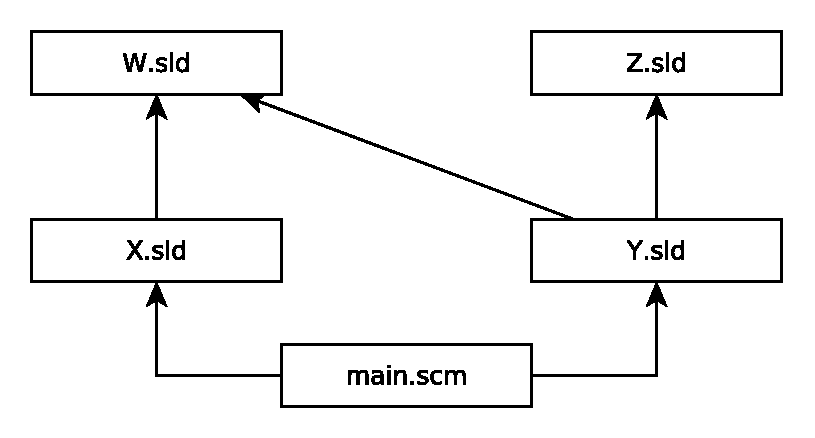
\includegraphics{figures/system-example}
  \caption{Un exemple d'un système fictif composé de différents modules.
  Le module principale se nomme utilise l'extension \textbf{.scm}
  et les bibliothèques porte l'extension \textbf{.sld}}
\end{figure} % TODO: use yed for that graph


Le démarrage du module principal Main.scm déclenche la collection des modules X
et Y, qui récursivement déclenche la collection de W et Z. L'algorithme de
collection des modules ignore les module qui apparaisse plusieurs fois au sein
du graphe.

Une fois la collection de tous ces modules est complété le descripteur de
module est récupéré par un appels à \verb|dlopen| et \verb|dlsym| dans le cas
compilé.


\section{Module hébergé}

Un module qui est hébergé est un module qui dont son contenu
se retrouve sur un domain comme \url{github.com}.


\begin{figure}[ht]
\begin{lstlisting}
hostname      = +( domainlabel "." ) toplabel
domainlabel   = alphanum | alphanum *( alphanum | "-" ) alphanum
toplabel      = alpha | alpha *( alphanum | "-" ) alphanum
alphanum      = alpha | digit
alpha         = [a-zA-Z]
digit         = [0-9]
\end{lstlisting}
  \caption{Grammaire BNF représentant un hostname selon un sous
  ensemble du RFC-2396.}
\end{figure}

La différence avec la spécification du hostname dans le RFC-2396
est que le hostname ne peut pas finir par un point et doit contenir
au moins un \verb|domainlabel|. C'est pour permettre de distingué
un module local et un module hébergé.

\subsection{Module gambit/git}

Ce module offre un interface pour utiliser interagir avec les des dépôts git.
Il permet de cloner un dépôts qui est hébergé sur \url{github.com}. Un clone du
dépôts est simplement un copie qui contient les informations suffisantes pour
passer d'une version d'un module à un autre. L'opération qui permet de changer
de version est \emph{checkout}.


%-------------------------------------------------------------------------------
%
%Modèle "link dynamique" :
%  recherche des libs au run time, utilisation de eval (par load) et
%  load-object-file
%
%  % gsi main.scm      ou      % gsc main.scm ; gsi main.o1
%
%    origin/main.scm    : (import X Y)
%          /X/X.sld     : (import)
%
% ~~userlib/Y/Y.sld     : (import Z)
%
%     ~~lib/Z/Z.sld     : (import)
%          /Z.o1
%
%-------------------------------------------------------------------------------
%
%Modèle "link statique" :
%  recherche des libs au link time en utilisant les méta-infos
%  dans les .c (demand-lib et supply-lib), chaque .c compilé en
%  un .o séparément et les .o linkés par le compilateur C
%
%  % gsc -obj -keep-c X.sld      ;; créer .c et .o
%  % gsc -obj -keep-c Y.sld      ;; créer .c et .o
%  % gsc -obj -keep-c Z.sld      ;; créer .c et .o
%  % gsc -obj -keep-c main.scm   ;; créer .c et .o
%  % gsc -exe main.c             ;; combine les .o pour créer main.exe
%
%    origin/main.scm    : (import X Y)
%          /main.c      : (demand-lib X Y)
%          /main.o
%          /X/X.sld     : (import)
%            /X.c       : (demand-lib) (supply-lib X)
%            /X.o
%
% ~~userlib/Y/Y.sld     : (import Z)
%          /Y/Y.c       : (demand-lib Z) (supply-lib Y)
%          /Y/Y.o
%
%     ~~lib/Z/Z.sld     : (import)
%          /Z/Z.c       : (demand-lib) (supply-lib Z)
%          /Z/Z.o
%
%-------------------------------------------------------------------------------
%
%Modèle "whole-program" :
%  recherche des libs au compile time en utilisant les imports
%  dans les fichiers sources, les AST de toutes les libs fusionnées
%  en un seul AST compilé par gsc (donc un seul .c généré et compilé
%  par le compilateur C pour créer main.exe)
%
%  % gsc -exe -whole-program main.scm
%
%    origin/main.scm    : (import X Y)
%          /X/X.sld     : (import)
%
% ~~userlib/Y/Y.sld     : (import Z)
%
%     ~~lib/Z/Z.sld     : (import)
%
%-------------------------------------------------------------------------------
% correction d’une petite coquille…
% /Y.c       : (demand-lib Z) (supply-lib Y)
% /Y.o
%
% ~~lib/Z/Z.sld     : (import)
% /Z.c       : (demand-lib) (supply-lib Z)
% ...


% (check-sld "/tmp/scheme/base/base.sld" "/tmp/scheme/base")
% (check-sld "/tmp/scheme/base.sld" "/tmp/scheme")
% (check-sld
%  "/home/frederic/Documents/MasterResearch/gambit9/lib/cocolappin/scheme/base/base.sld"
%  "/home/frederic/Documents/MasterResearch/gambit9/lib/cocolappin/scheme/base")
% (check-sld
%  "/home/frederic/Documents/MasterResearch/gambit9/lib/cocolappin/scheme/base.sld"
%  "/home/frederic/Documents/MasterResearch/gambit9/lib/cocolappin/scheme")
% (check-sld
%  "/home/frederic/Documents/MasterResearch/g9/lib/scheme/base/base.sld"
%  "/home/frederic/Documents/MasterResearch/g9/lib/scheme/base")
% object-file-path: /home/frederic/Documents/MasterResearch/g9/lib/scheme/base/.gambit_409003@C/base.o1
% ("/home/frederic/Documents/MasterResearch/g9/lib/scheme/base/base.sld"
%  .
%  #<input-port #2 "/home/frederic/Documents/MasterResearch/g9/lib/scheme/base/base.sld">)
